\documentclass[10pt,ignorenonframetext,,aspectratio=149]{beamer}
\usefonttheme{serif} % use mainfont rather than sansfont for slide text
\setbeamertemplate{caption}[numbered]
\setbeamertemplate{caption label separator}{: }
\setbeamercolor{caption name}{fg=normal text.fg}
\usepackage{lmodern}
\usepackage{amssymb,amsmath}
\usepackage{ifxetex,ifluatex}
\usepackage{fixltx2e} % provides \textsubscript
\ifnum 0\ifxetex 1\fi\ifluatex 1\fi=0 % if pdftex
  \usepackage[T1]{fontenc}
  \usepackage[utf8]{inputenc}
\else % if luatex or xelatex
  \ifxetex
    \usepackage{mathspec}
  \else
    \usepackage{fontspec}
  \fi
  \defaultfontfeatures{Ligatures=TeX,Scale=MatchLowercase}
  \newcommand{\euro}{€}
    \setmainfont[]{Open Sans}
\fi
% use upquote if available, for straight quotes in verbatim environments
\IfFileExists{upquote.sty}{\usepackage{upquote}}{}
% use microtype if available
\IfFileExists{microtype.sty}{%
\usepackage{microtype}
\UseMicrotypeSet[protrusion]{basicmath} % disable protrusion for tt fonts
}{}
\usepackage{graphicx,grffile}
\makeatletter
\def\maxwidth{\ifdim\Gin@nat@width>\linewidth\linewidth\else\Gin@nat@width\fi}
\def\maxheight{\ifdim\Gin@nat@height>\textheight0.8\textheight\else\Gin@nat@height\fi}
\makeatother
% Scale images if necessary, so that they will not overflow the page
% margins by default, and it is still possible to overwrite the defaults
% using explicit options in \includegraphics[width, height, ...]{}
\setkeys{Gin}{width=\maxwidth,height=\maxheight,keepaspectratio}

% Comment these out if you don't want a slide with just the
% part/section/subsection/subsubsection title:
\AtBeginPart{
  \let\insertpartnumber\relax
  \let\partname\relax
  \frame{\partpage}
}
\AtBeginSection{
  \let\insertsectionnumber\relax
  \let\sectionname\relax
  \frame{\sectionpage}
}
\AtBeginSubsection{
  \let\insertsubsectionnumber\relax
  \let\subsectionname\relax
  \frame{\subsectionpage}
}

\setlength{\emergencystretch}{3em}  % prevent overfull lines
\providecommand{\tightlist}{%
  \setlength{\itemsep}{0pt}\setlength{\parskip}{0pt}}
\setcounter{secnumdepth}{0}

\title{Estimating the Regression Model by Least Squares}
\author{Henrique Veras}
\date{}

%% Here's everything I added.
%%--------------------------

\usepackage{graphicx}
\usepackage{rotating}
%\setbeamertemplate{caption}[numbered]
\usepackage{hyperref}
\usepackage{caption}
\usepackage[normalem]{ulem}
%\mode<presentation>
\usepackage{wasysym}
%\usepackage{amsmath}


% Get rid of navigation symbols.
%-------------------------------
\setbeamertemplate{navigation symbols}{}

% Optional institute tags and titlegraphic.
% Do feel free to change the titlegraphic if you don't want it as a Markdown field.
%----------------------------------------------------------------------------------
\institute{PIMES/UFPE}

% \titlegraphic{\includegraphics[width=0.3\paperwidth]{\string~/Dropbox/teaching/clemson-academic.png}} % <-- if you want to know what this looks like without it as a Markdown field. 
% -----------------------------------------------------------------------------------------------------


% Some additional title page adjustments.
%----------------------------------------
\setbeamertemplate{title page}[empty]
%\date{}
\setbeamerfont{subtitle}{size=\small}

\setbeamercovered{transparent}

% Some optional colors. Change or add as you see fit.
%---------------------------------------------------
\definecolor{clemsonpurple}{HTML}{522D80}
 \definecolor{clemsonorange}{HTML}{F66733}
\definecolor{uiucblue}{HTML}{003C7D}
\definecolor{uiucorange}{HTML}{F47F24}


% Some optional color adjustments to Beamer. Change as you see fit.
%------------------------------------------------------------------
\setbeamercolor{frametitle}{fg=clemsonpurple,bg=white}
\setbeamercolor{title}{fg=clemsonpurple,bg=white}
\setbeamercolor{local structure}{fg=clemsonpurple}
\setbeamercolor{section in toc}{fg=clemsonpurple,bg=white}
% \setbeamercolor{subsection in toc}{fg=clemsonorange,bg=white}
\setbeamercolor{footline}{fg=clemsonpurple!50, bg=white}
\setbeamercolor{block title}{fg=clemsonorange,bg=white}


\let\Tiny=\tiny


% Sections and subsections should not get their own damn slide.
%--------------------------------------------------------------
\AtBeginPart{}
\AtBeginSection{}
\AtBeginSubsection{}
\AtBeginSubsubsection{}

% Suppress some of Markdown's weird default vertical spacing.
%------------------------------------------------------------
\setlength{\emergencystretch}{0em}  % prevent overfull lines
\setlength{\parskip}{0pt}


% Allow for those simple two-tone footlines I like. 
% Edit the colors as you see fit.
%--------------------------------------------------
\defbeamertemplate*{footline}{my footline}{%
    \ifnum\insertpagenumber=1
    \hbox{%
        \begin{beamercolorbox}[wd=\paperwidth,ht=.8ex,dp=1ex,center]{}%
      % empty environment to raise height
        \end{beamercolorbox}%
    }%
    \vskip0pt%
    \else%
        \Tiny{%
            \hfill%
		\vspace*{1pt}%
            \insertframenumber/\inserttotalframenumber \hspace*{0.1cm}%
            \newline%
            \color{clemsonpurple}{\rule{\paperwidth}{0.4mm}}\newline%
            \color{clemsonorange}{\rule{\paperwidth}{.4mm}}%
        }%
    \fi%
}

% Various cosmetic things, though I must confess I forget what exactly these do and why I included them.
%-------------------------------------------------------------------------------------------------------
\setbeamercolor{structure}{fg=blue}
\setbeamercolor{local structure}{parent=structure}
\setbeamercolor{item projected}{parent=item,use=item,fg=clemsonpurple,bg=white}
\setbeamercolor{enumerate item}{parent=item}

% Adjust some item elements. More cosmetic things.
%-------------------------------------------------
\setbeamertemplate{itemize item}{\color{clemsonpurple}$\bullet$}
\setbeamertemplate{itemize subitem}{\color{clemsonpurple}\scriptsize{$\bullet$}}
\setbeamertemplate{itemize/enumerate body end}{\vspace{.6\baselineskip}} % So I'm less inclined to use \medskip and \bigskip in Markdown.

% Automatically center images
% ---------------------------
% Note: this is for ![](image.png) images
% Use "fig.align = "center" for R chunks

\usepackage{etoolbox}

\AtBeginDocument{%
  \letcs\oig{@orig\string\includegraphics}%
  \renewcommand<>\includegraphics[2][]{%
    \only#3{%
      {\centering\oig[{#1}]{#2}\par}%
    }%
  }%
}

% I think I've moved to xelatex now. Here's some stuff for that.
% --------------------------------------------------------------
% I could customize/generalize this more but the truth is it works for my circumstances.

\ifxetex
\setbeamerfont{title}{family=\fontspec{Titillium Web}}
\setbeamerfont{frametitle}{family=\fontspec{Titillium Web}}
\usepackage[font=small,skip=0pt]{caption}
 \else
 \fi

% Okay, and begin the actual document...

\begin{document}
\frame{\titlepage}

\hypertarget{econometrics}{%
\section{Econometrics}\label{econometrics}}

\hypertarget{intro}{%
\subsection{Intro}\label{intro}}

\begin{frame}{Today}
\protect\hypertarget{today}{}
We now examine the Least Squares as an \textbf{estimator} of the
parameters of the linear regression model.

\vfill

We start by analysing the question ``\emph{why should we use least
squares}''?

\vfill

We will compare the LS estimator to other candidates based on their
\textbf{statistical properties}:

\begin{enumerate}
\tightlist
\item
  Unbiasedness
\item
  Efficiency
\item
  Consistency
\end{enumerate}

\vfill
\end{frame}

\hypertarget{population-orthogonality-conditions}{%
\subsection{Population orthogonality
conditions}\label{population-orthogonality-conditions}}

\begin{frame}{Population orthogonality}
\protect\hypertarget{population-orthogonality}{}
Recall assumption A3: \(E[\varepsilon_i|\mathbf{X}]=0\)

\vfill

By iterated expectations,
\(E[\varepsilon]= E_x {E[\varepsilon_i|\mathbf{X}]}=E_x[0]=0\).

\vfill

Also,
\(cov(\mathbf{x}, \mathbf{\varepsilon})=cov[\mathbf{x}, E[\varepsilon_i|\mathbf{X}]]=cov(\mathbf{x},0)=0\),
so \(\mathbf{x}\) and \(\mathbf{\varepsilon}\) are uncorrelated.

\vfill

From these results we can find that
\[E[\mathbf{Xy}]=E[\mathbf{X'X}]\mathbf{\beta}\]

\vfill
\end{frame}

\begin{frame}{Population orthogonality}
\protect\hypertarget{population-orthogonality-1}{}
Now recall the FOC of the LS problem: \(\mathbf{X'y}=\mathbf{X'Xb}\).
Dividing both sides by \(n\) and writing it as a summation:

\[\frac{1}{n}\sum_{i=1}^n{\mathbf{x_i y_i}}=\left(\frac{1}{n}\sum_{i=1}^n{\mathbf{x_i'x_i}}\right)\mathbf{b}\]

\vfill

Notice that this is the sample counterpart of the population condition
\(E[\mathbf{Xy}]=E[\mathbf{X'X}]\mathbf{\beta}\).
\end{frame}

\hypertarget{statistical-properties-of-the-ls-estimator}{%
\subsection{Statistical Properties of the LS
Estimator}\label{statistical-properties-of-the-ls-estimator}}

\begin{frame}{Statistical Properties of the LS Estimator}
\protect\hypertarget{statistical-properties-of-the-ls-estimator-1}{}
An \textbf{estimator} is a strategy for using the sample data that are
drawn from a population.

\vfill

The \textbf{properties} of that estimator are descriptions of how it can
be expected to behave when it is appied to a sample of data.
\end{frame}

\begin{frame}{Unbiasedness}
\protect\hypertarget{unbiasedness}{}
The least squares estimator is \textbf{unbiased} in every sample:

\vfill

\[E[\mathbf{b}|\mathbf{X}]=\mathbf{\beta}\]

Moreover,

\[E[\mathbf{b}]=E_x[E[\mathbf{b}|\mathbf{X}]]=E_x[\mathbf{\beta}]=\mathbf{\beta}\]

\vfill

This is to say that the Least Squares estimator has expectation
\(\mathbf{\beta}\).

\vfill

Moreover, when we average this over the possible values of
\(\mathbf{X}\), the unconditional mean is also \(\mathbf{\beta}\).

\vfill
\end{frame}

\begin{frame}{Omitted Variable Bias (OVB)}
\protect\hypertarget{omitted-variable-bias-ovb}{}
Suppose the true population model is given by
\[\mathbf{y}=\mathbf{X\beta}+\gamma z + \mathbf{\varepsilon}\]

\vfill

If we estimate \(\mathbf{y}\) on \(\mathbf{X}\) only, without the
\emph{relevant} variable \(z\), the estimator is

\[\begin{split}
\mathbf{b} & =(\mathbf{X}'\mathbf{X})^{-1}\mathbf{X}'\mathbf{y}=(\mathbf{X}'\mathbf{X})^{-1}\mathbf{X}'(\mathbf{X\beta}+\gamma z+\varepsilon) \\
 & = \mathbf{\beta}+(\mathbf{X}'\mathbf{X})^{-1}\mathbf{X}'\gamma z+(\mathbf{X}'\mathbf{X})^{-1}\mathbf{X}'\mathbf{\varepsilon}
 \end{split}\]

\vfill
\end{frame}

\begin{frame}{Omitted Variable Bias (OVB)}
\protect\hypertarget{omitted-variable-bias-ovb-1}{}
The expected value is given by

\[\begin{split}
E[\mathbf{b}|\mathbf{X},z] & =\mathbf{\beta}+(\mathbf{X}'\mathbf{X})^{-1}\mathbf{X}' \gamma z\\
 & = \mathbf{\beta} + \mathbf{p}_{X.z}\gamma,
\end{split}\]

where \(\mathbf{p}_{X.z}=(\mathbf{X}'\mathbf{X})^{-1}\mathbf{X}'z\).
What does it represent? What happens if \(\mathbf{X}\) and z are
orthogonal?

\vfill

Based on the FWL theorem and corollary 3.2.1, we can write

\[E[b_k|\mathbf{X},z]=\beta_k+\gamma\left(\frac{cov(z, x_k| \text{all other x's})}{var(x_k | \text{all other x's})}\right)\]

\vfill
\end{frame}

\begin{frame}{An Example}
\protect\hypertarget{an-example}{}
Suppose we are interested in estimating the returns to education
regression model below:

\[Income=\beta_0+\beta_1 Educ + \beta_2 age + \beta_3 age^2 + \beta_4 Abil + \varepsilon\]

\vfill

What is the sign of the bias if we estimate the model above without the
(\emph{unobserved}) \(Abil\)?

\vfill
\end{frame}

\begin{frame}{An Example}
\protect\hypertarget{an-example-1}{}
The sign of the bias will depend on the signs of \(\gamma\) and
\(cov(z, x_k| \text{all other x's})\):

\[E[b_1|\mathbf{X},z]=\beta_1+\gamma\left(\frac{cov(Abil, Educ | age, age^2)}{var(Educ | age, age^2)}\right)\]

\vfill

Thus, if \(\gamma>0\) and \(cov(Abil, Educ | age, age^2)>0\), \(b_1\)
will be biased upward: \[E[b_1|\mathbf{X},z]>\beta_1\]

\vfill

Notice, however, that in some circumstances, the sign of the conditional
covariance might not be obvious!

\vfill

What happens if we include irrelevant variables instead?
\end{frame}

\begin{frame}{Variance of the Least Squares Estimator}
\protect\hypertarget{variance-of-the-least-squares-estimator}{}
If Assumption A4 holds, the variance of the Least Squares estimator is
given by

\[Var(\mathbf{b}|\mathbf{X})=\sigma^2(\mathbf{X'X})^{-1}\]

\vfill

If we wish to find a sample estimate of \(Var(\mathbf{b}|\mathbf{X})\),
we need to estimate the (unknown) population parameter \(\sigma^2\).

\vfill

Recall:

\begin{enumerate}
\tightlist
\item
  \(\sigma^2\) is the variance of the error term:
  \(\sigma^2=E[\varepsilon_i^2|\mathbf{X}]\)
\item
  \(e_i\) is the estimate of \(\varepsilon_i\)
\end{enumerate}

\vfill
\end{frame}

\begin{frame}{Variance of the Least Squares Estimator}
\protect\hypertarget{variance-of-the-least-squares-estimator-1}{}
A natural estimator for \(\sigma^2\) would then be
\(\hat{\sigma}^2=\frac{1}{n} \sum_{i=1}^n{e_i^2}\).

\vfill

However, we would also need to estimate \(K\) parameters
\(\mathbf{\beta}\), which would distort \(\sigma^2\).

\vfill

An \textbf{unbiased} estimator for \(\sigma^2\) is
\[s^2=\frac{\mathbf{e}'\mathbf{e}}{n-K}\]

\vfill

Like \(\mathbf{b}\), \(s^2\) is unbiased unconditionally because
\[E[s^2]=E_X[E[s^2|\mathbf{X}]]=E_X[\sigma^2]=\sigma^2\]
\end{frame}

\begin{frame}{Variance of the Least Squares Estimator}
\protect\hypertarget{variance-of-the-least-squares-estimator-2}{}
The \textbf{standard error of the regression} is \(s=\sqrt{s^2}\).

\vfill

The variance of the Least Squares Estimator can thus be estimated by

\[\hat{Var}(\mathbf{b}|X)=s^2(\mathbf{X'X})^{-1}\]

\vfill

\(\hat{Var}(\mathbf{b}|X)\) is the sample estimate of the \emph{sampling
variance} of the LS estimator.

\vfill

Notice that the \(k\)-th diagonal element of this matrix is
\([s^2(\mathbf{X'X}_{kk})^{-1}]^{1/2}\), the standard error of the
estimator \(b_k\).
\end{frame}

\hypertarget{the-gauss-markov-theorem}{%
\subsection{The Gauss-Markov Theorem}\label{the-gauss-markov-theorem}}

\begin{frame}{The Gauss-Markov Theorem}
\protect\hypertarget{the-gauss-markov-theorem-1}{}
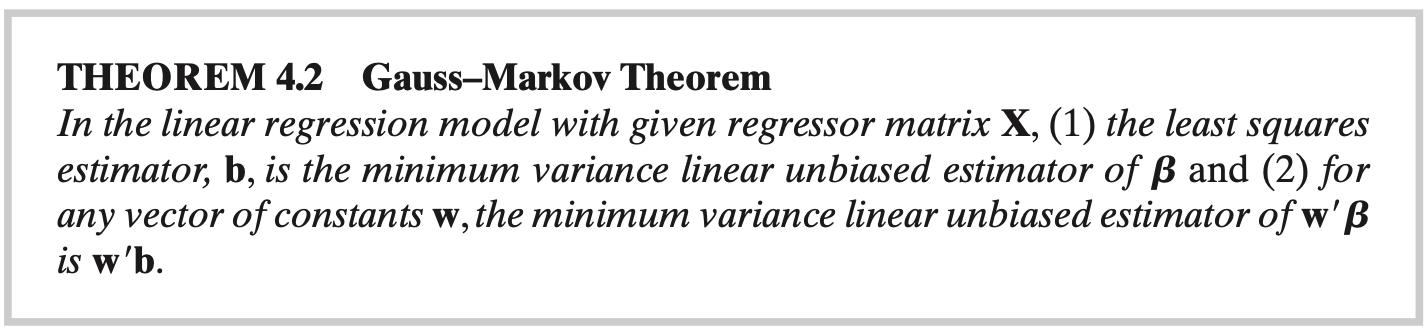
\includegraphics{/Users/henriquefonseca/Desktop/temp/Rmarkdown-practice/henriqueveras.github.io/files/Econometrics/Lecture Notes/3/theorem_4.2.png}
\end{frame}

\begin{frame}{The Normality Assumption}
\protect\hypertarget{the-normality-assumption}{}
We have not used assumption A6 until now. Recall:

\vfill

\(\mathbf{b}=\mathbf{\beta}+(\mathbf{X}'\mathbf{X})^{-1}\mathbf{X}'\mathbf{\varepsilon}\)

\vfill

If \textbf{Assumption A6} is satisfied:
\(\varepsilon|\mathbf{X} \sim N(\mathbf{0},\sigma^2\mathbf{I})\)

\vfill

Thus,
\(\mathbf{b}|\mathbf{X} \sim N(\mathbf{\beta},\sigma^2(\mathbf{X}'\mathbf{X})^{-1})\)
\end{frame}

\hypertarget{asymptotic-properties-of-the-least-squares-estimator}{%
\subsection{Asymptotic Properties of the Least Squares
Estimator}\label{asymptotic-properties-of-the-least-squares-estimator}}

\begin{frame}{Asymptotic Properties of the Least Squares Estimator}
\protect\hypertarget{asymptotic-properties-of-the-least-squares-estimator-1}{}
The properties described above can be applied to any sample size
(\emph{finite sample} properties)

\vfill

Issues:

\begin{enumerate}
\tightlist
\item
  The list of settings in which exact finite sample results can be
  obtained is extremely small.
\item
  The assumption of normality likewise narrows the range of the
  applications.
\end{enumerate}

\vfill

We now extend our analysis to large samples. We might be able to obtain
more general approximate results.

\vfill
\end{frame}

\begin{frame}{Asymptotic Properties of the Least Squares Estimator}
\protect\hypertarget{asymptotic-properties-of-the-least-squares-estimator-2}{}
Unbiasedness has two important limitations:

\begin{enumerate}
\tightlist
\item
  It is rare for an econometric estimator to be unbiased (with the clear
  exception of the LS)
\item
  Does not imply that more data is better.
\end{enumerate}

\vfill

Throughout we'll rely on two crucial assumptions:

\begin{enumerate}
\tightlist
\item
  \textbf{A5a}: \((\mathbf{x}_i\mathbf{\varepsilon}_i), i=1,\cdots, n\),
  is a sequence of independent, identically distributed
  \emph{observations}.
\item
  \textbf{A2'}:
  \(\text{plim } \frac{(\mathbf{X}'\mathbf{X})}{n}=\mathbf{Q}\), a
  positive definite matrix.
\end{enumerate}

\vfill

Recall:

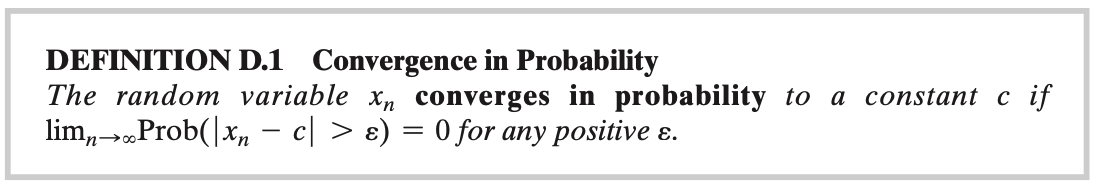
\includegraphics{/Users/henriquefonseca/Desktop/temp/Rmarkdown-practice/henriqueveras.github.io/files/Econometrics/Lecture Notes/3/definition_d.1.png}

\vfill

If \(x_n\) converges in probability to \(c\), then, we say that
\(\text{plim } x_n = c\).

\vfill
\end{frame}

\begin{frame}{Asymptotic Assumptions about \(\mathbf{X}\)}
\protect\hypertarget{asymptotic-assumptions-about-mathbfx}{}
At many points from here forward, we will make an assumption that the
data are \emph{well behaved} so that an estimator or statistic will
converge to a result.

\vfill

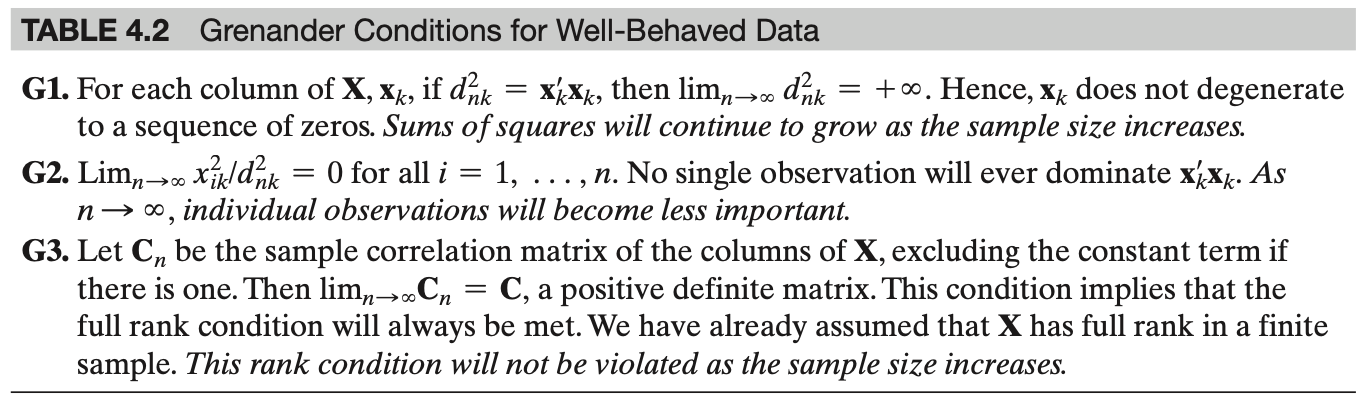
\includegraphics{/Users/henriquefonseca/Desktop/temp/Rmarkdown-practice/henriqueveras.github.io/files/Econometrics/Lecture Notes/3/table_4.2.png}
\end{frame}

\begin{frame}{Consistency of the LS estimator of \(\beta\)}
\protect\hypertarget{consistency-of-the-ls-estimator-of-beta}{}
Recall the general definition of consistency of an estimator:

\vfill

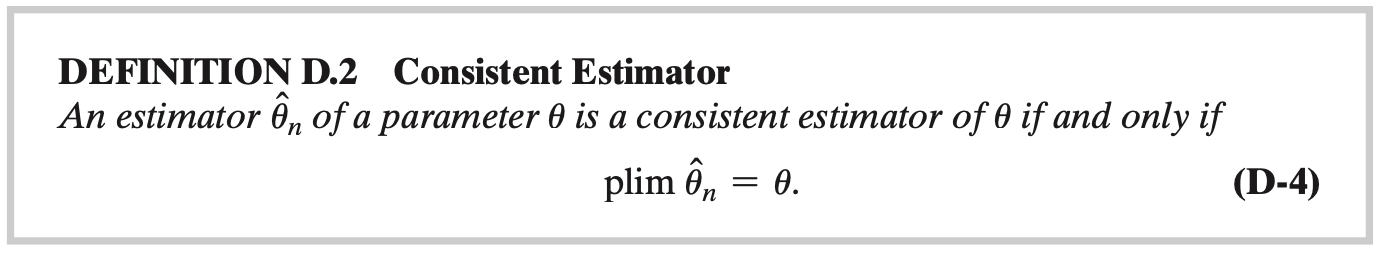
\includegraphics{/Users/henriquefonseca/Desktop/temp/Rmarkdown-practice/henriqueveras.github.io/files/Econometrics/Lecture Notes/3/definition_d.2.png}

\vfill

We will show that the LS estimator \(\mathbf{b}\) is consistent, that
is, \(\text{plim } \mathbf{b}= \mathbf{\beta}\).

\vfill

We can write \(\mathbf{b}\) as

\[\mathbf{b}=\mathbf{\beta}+\left(\frac{\mathbf{X}'\mathbf{X}}{n}\right)^{-1}\left(\frac{\mathbf{X}'\mathbf{\varepsilon}}{n}\right)\]

\vfill
\end{frame}

\begin{frame}{Some useful results}
\protect\hypertarget{some-useful-results}{}
Before proceeding to the consistency proof, recall some important
results:

\vfill

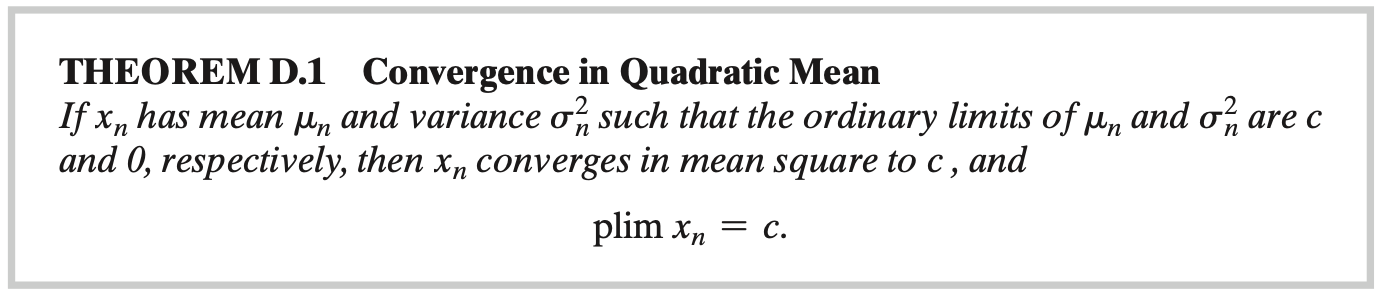
\includegraphics{/Users/henriquefonseca/Desktop/temp/Rmarkdown-practice/henriqueveras.github.io/files/Econometrics/Lecture Notes/3/theorem_d.1.png}

\vfill

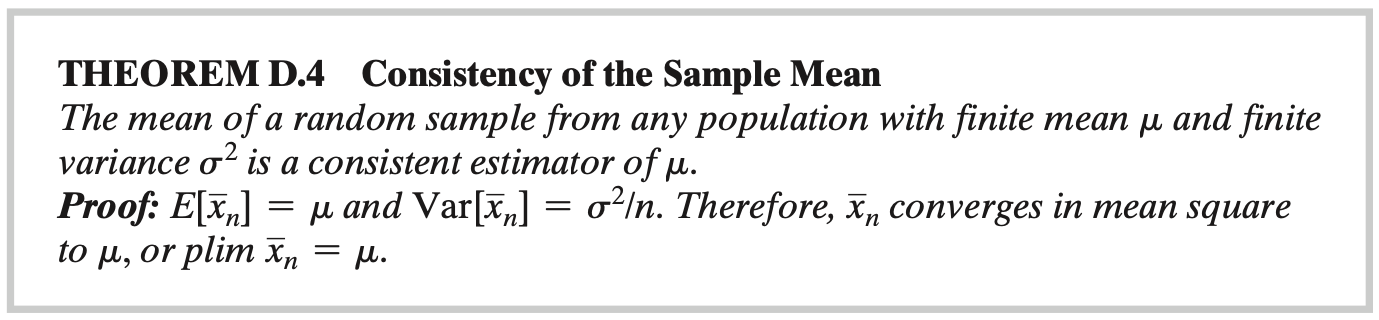
\includegraphics{/Users/henriquefonseca/Desktop/temp/Rmarkdown-practice/henriqueveras.github.io/files/Econometrics/Lecture Notes/3/theorem_d.4.png}

\vfill
\end{frame}

\begin{frame}{Some useful results}
\protect\hypertarget{some-useful-results-1}{}
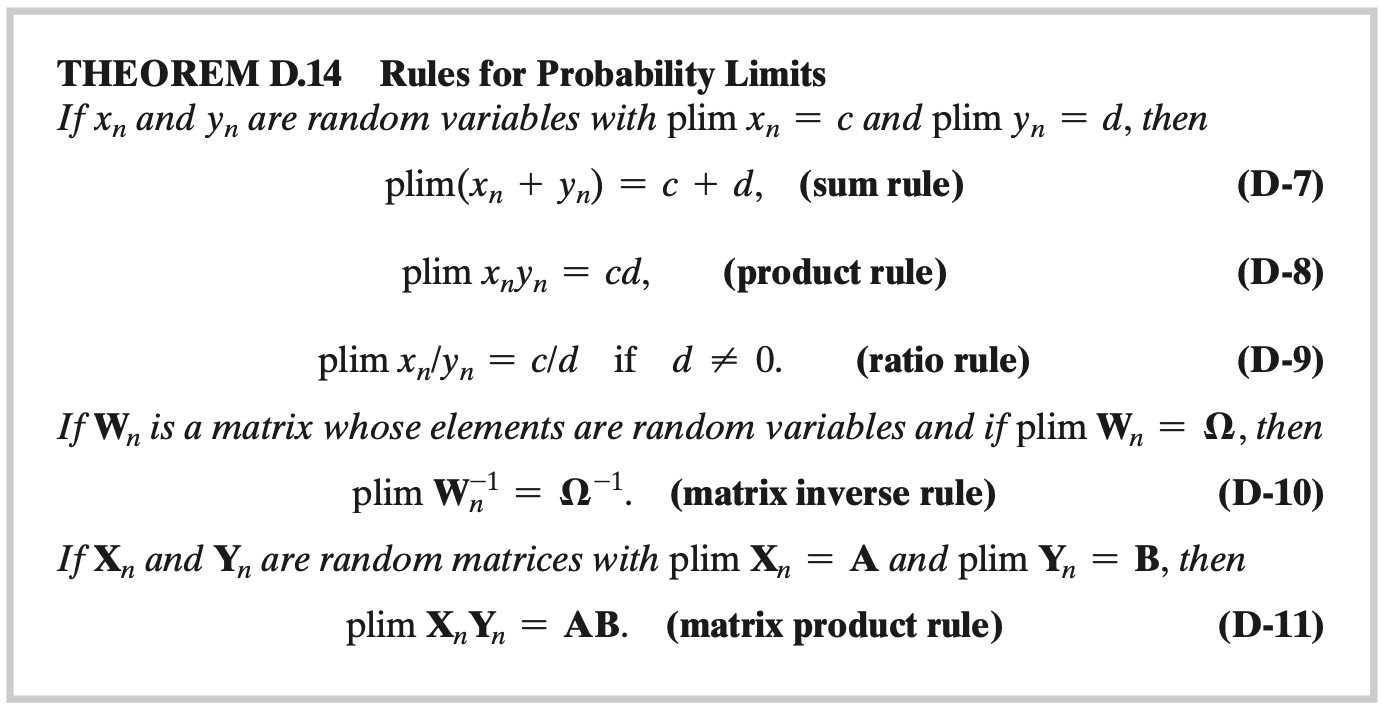
\includegraphics{/Users/henriquefonseca/Desktop/temp/Rmarkdown-practice/henriqueveras.github.io/files/Econometrics/Lecture Notes/3/theorem_d.14.png}
\end{frame}

\begin{frame}{Consistency of the LS estimator of \(\beta\)}
\protect\hypertarget{consistency-of-the-ls-estimator-of-beta-1}{}
Now, the probability limit of \(\mathbf{b}\) is

\[\text{plim } \mathbf{b}=\mathbf{\beta}+\mathbf{Q}^{-1}\text{plim }\left(\frac{\mathbf{X}'\mathbf{\varepsilon}}{n}\right)\]

To find \(\text{plim } \mathbf{b}\), we need to check
\(\text{plim }\left(\frac{\mathbf{X}'\mathbf{\varepsilon}}{n}\right)\):

\vfill

According to Theorem D.4, the sample mean is a consistent estimator of
the population mean. therefore

\[\frac{\mathbf{X}'\mathbf{\varepsilon}}{n}=\frac{1}{n}\sum_{i=1}^n{\mathbf{x}_i\varepsilon_i}\]

converges in probability to its expected value,
\(E[\mathbf{\varepsilon}\mathbf{X}]\), which is zero (why?).

\vfill
\end{frame}

\begin{frame}{Consistency of the LS estimator of \(\beta\)}
\protect\hypertarget{consistency-of-the-ls-estimator-of-beta-2}{}
It follows that
\(\text{plim }\left(\frac{\mathbf{X}'\mathbf{\varepsilon}}{n}\right)=0\)

\vfill

Thus, \(\text{plim } \mathbf{b}=\mathbf{\beta}\).

\vfill

For any individual coefficient of the vector \(\mathbf{b}\), we have

\[\lim_{n\to\infty} Prob[|b_k-\beta_k|>\delta]=0\]

for any \(\delta>0\)

\vfill
\end{frame}

\begin{frame}{The Estimator of the \(Asy. Var[\mathbf{b}]\)}
\protect\hypertarget{the-estimator-of-the-asy.-varmathbfb}{}
To complete the derivation of the asymptotic properties of
\(\mathbf{b}\), we will require an estimator of
\(Asy. Var[\mathbf{b}]=\sigma^2/n\mathbf{Q}^{-1}\), provided that
\textbf{A2'} is satisfied.

\vfill

It can be shown that \(s^2\) is a \textbf{consistent} estimator of
\(\sigma^2\). (you should be able to show this!)

\vfill

Thus, by the product rule of the probability limits, we have

\[\text{plim } s^2(\mathbf{X}'\mathbf{X}/n)^{-1}=\sigma^2\mathbf{Q}^{-1}\]

\vfill

The appropriate estimator of the asymptotic covariance matrix of
\(\mathbf{b}\) is

\[Est.Asy.Var [\mathbf{b}]=s^2(\mathbf{X}'\mathbf{X})^{-1}\]
\end{frame}

\begin{frame}{Asymptotic Normality of the Least Squares Estimator}
\protect\hypertarget{asymptotic-normality-of-the-least-squares-estimator}{}
Let us now derive the asymptotic distribution of the Least Squares
estimator.

\vfill

Notice that we do not require that \textbf{A6} is satisfied here. If it
is, then the sampling distribution of \(\mathbf{b}\) is \emph{exact}
normal for every sample, which also holds asymptotically.

\vfill

We now rewrite \(\mathbf{b}\) as

\[\mathbf{b}-\mathbf{\beta}=\left(\frac{\mathbf{X}'\mathbf{X}}{n}\right)^{-1}\left(\frac{\mathbf{X}'\mathbf{\varepsilon}}{n}\right)\]

A multivariate version of the following theorem can be useful:

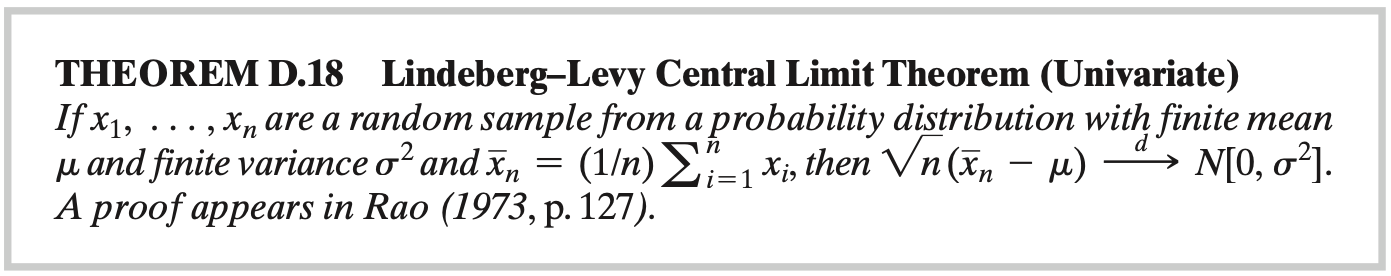
\includegraphics{/Users/henriquefonseca/Desktop/temp/Rmarkdown-practice/henriqueveras.github.io/files/Econometrics/Lecture Notes/3/theorem_d.18.png}
\end{frame}

\begin{frame}{Asymptotic Normality of the Least Squares Estimator}
\protect\hypertarget{asymptotic-normality-of-the-least-squares-estimator-1}{}
Multiplying both sides by \(\sqrt{n}\):

\[\sqrt{n}(\mathbf{b}-\mathbf{\beta})=\left(\frac{\mathbf{X}'\mathbf{X}}{n}\right)^{-1}\left(\frac{1}{\sqrt{n}}\right)\mathbf{X}'\mathbf{\varepsilon}\]
\vfill

As we know that
\(\text{plim } \left(\frac{\mathbf{X}'\mathbf{X}}{n}\right)^{-1}=\mathbf{Q}^{-1}\),
the \emph{limiting} distribution of
\(\sqrt{n}(\mathbf{b}-\mathbf{\beta})\) is the same as the limiting
distribution of

\[\mathbf{Q}^{-1}\frac{1}{\sqrt{n}}\mathbf{X}'\mathbf{\varepsilon}\]

\vfill
\end{frame}

\begin{frame}{Asymptotic Normality of the Least Squares Estimator}
\protect\hypertarget{asymptotic-normality-of-the-least-squares-estimator-2}{}
We can show that \(\frac{1}{\sqrt{n}}\mathbf{X}'\mathbf{\varepsilon}\)
can be written as

\[\sqrt{n}[\bar{\mathbf{w}}-E(\bar{\mathbf{w}})],\]

where \(\mathbf{w}_i=\sum{\mathbf{x}_i\varepsilon_i}\) and
\(\bar{\mathbf{w}}=(1/n)\sum{\mathbf{w}_i}\).

\vfill

The vector \(\bar{\mathbf{w}}\) is the average of \(n\) \(i.i.d.\)
random vectors with mean \(0\) and variance
\(Var[\varepsilon_i\mathbf{x}_i]=\sigma^2E[\mathbf{x_ix_i'}]=\sigma^2\mathbf{Q}\).
\end{frame}

\begin{frame}{Asymptotic Normality of the Least Squares Estimator}
\protect\hypertarget{asymptotic-normality-of-the-least-squares-estimator-3}{}
We can show that the variance of
\(\sqrt{n}\bar{\mathbf{w}}=\sigma^2\mathbf{Q}\).

\vfill

Thus, applying the Lindeberg--Levy central limit theorem, if
\([\mathbf{x}_i\varepsilon_i]\), \(i=1,\cdots,n\), are independent
vectors, each distributed with mean 0 and variance
\(\sigma^2\mathbf{Q}<\infty\), and \textbf{A2'} holds, then

\[\left(\frac{1}{\sqrt{n}}\right)\mathbf{X}'\mathbf{\varepsilon}\xrightarrow{d}N[0,\sigma^2\mathbf{Q}]\]
\end{frame}

\begin{frame}{Asymptotic Normality of the Least Squares Estimator}
\protect\hypertarget{asymptotic-normality-of-the-least-squares-estimator-4}{}
From the previous result, we can find the following theorem:

\vfill

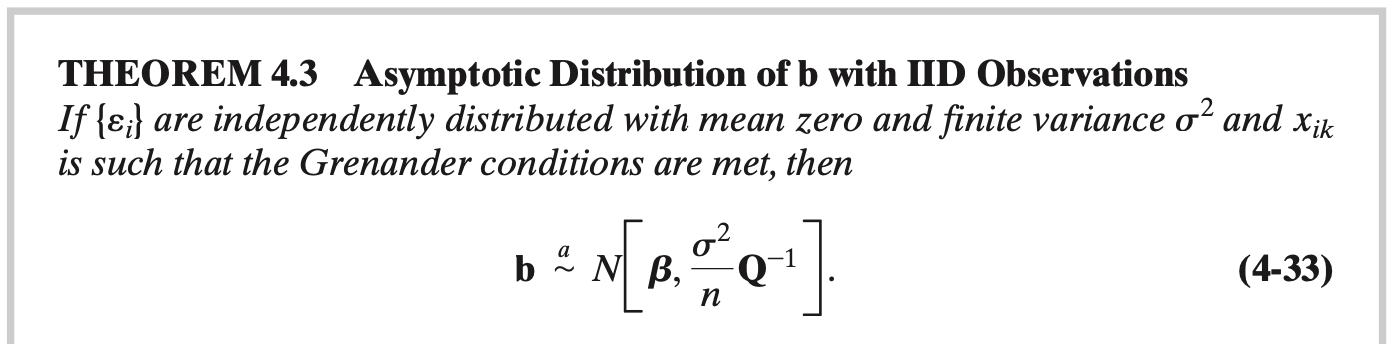
\includegraphics{/Users/henriquefonseca/Desktop/temp/Rmarkdown-practice/henriqueveras.github.io/files/Econometrics/Lecture Notes/3/theorem_4.3.png}

\vfill

In practice, we need to estimate \(\frac{1}{n}\mathbf{Q}^{-1}\) with
\((\mathbf{X'X})^{-1}\) and \(\sigma^2\) with
\(s^2=\frac{\mathbf{e'e}}{n-K}\).

\vfill
\end{frame}

\begin{frame}{Asymptotic Efficiency}
\protect\hypertarget{asymptotic-efficiency}{}
The Gauss-Markov Theorem establishes finite sample conditions under
which the LS estimator is optimal.

\vfill

The requirements that the estimator be \emph{linear} and \emph{unbiased}
limit the theorem's generality, however.

\vfill

In asymptotic theory, we are interested in expanding the scope of
analysis to estimators that might be biased but consistent.

\vfill

Moreover, we might also be interested in comparing non-linear estimators
as well.

\vfill
\end{frame}

\begin{frame}{Asymptotic Efficiency}
\protect\hypertarget{asymptotic-efficiency-1}{}
These cases extend beynd the reach of the Gauss-Marvok theorem.

\vfill

Below we present an alternative criterion:

\vfill

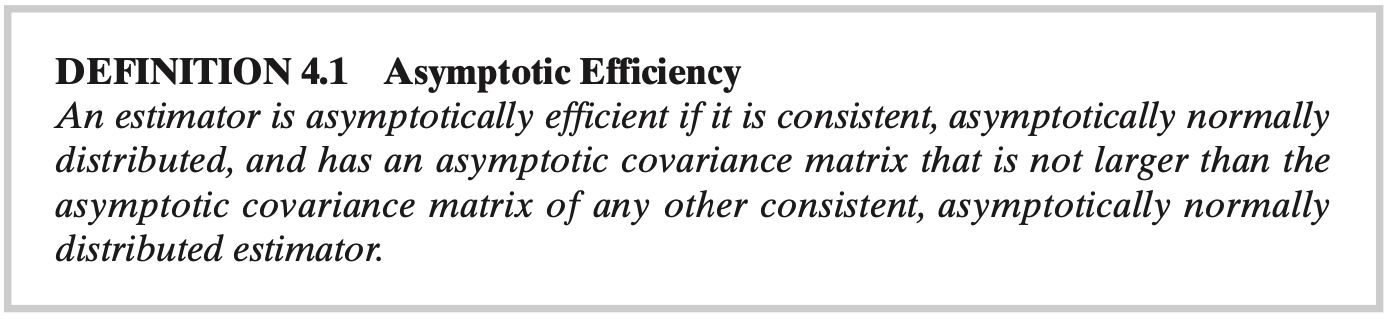
\includegraphics{/Users/henriquefonseca/Desktop/temp/Rmarkdown-practice/henriqueveras.github.io/files/Econometrics/Lecture Notes/3/definition_4.1.png}

\vfill
\end{frame}

\begin{frame}{Some comments on Asymptotic Efficiency}
\protect\hypertarget{some-comments-on-asymptotic-efficiency}{}
We can compare estimators based on their asymptotic variances.

\vfill

The complication in comparing two consistent estimators is that both
converge to the true parameter as the sample size increases.

\vfill

Moreover, it usually happens that they converge at the same rate---that
is, in both cases, the asymptotic variances of the two estimators are of
the same order.

\vfill

In such a situation, we can sometimes compare the asymptotic variances
for the same \(n\) to resolve the ranking.
\end{frame}

\hypertarget{the-delta-method}{%
\subsection{The Delta Method}\label{the-delta-method}}

\begin{frame}{Asymptotic Distribution of a Function of \(\mathbf{b}\):
The Delta Method}
\protect\hypertarget{asymptotic-distribution-of-a-function-of-mathbfb-the-delta-method}{}
Let \(\mathbf{b}\) be a set of \(J\) continuous, linear or non-linear,
and continuously differentiable functions of the LS estimators and let

\[\mathbf{C}(\mathbf{b})=\frac{\partial f(\mathbf{b})}{\partial \mathbf{b}'}\]
a \(J\times K\) matrix whose \(j\)th row is the vector of derivatives of
the \(j\)th function with respect to \(\mathbf{b}'\).

\vfill

We'll use the Slutsky theorem:

\vfill

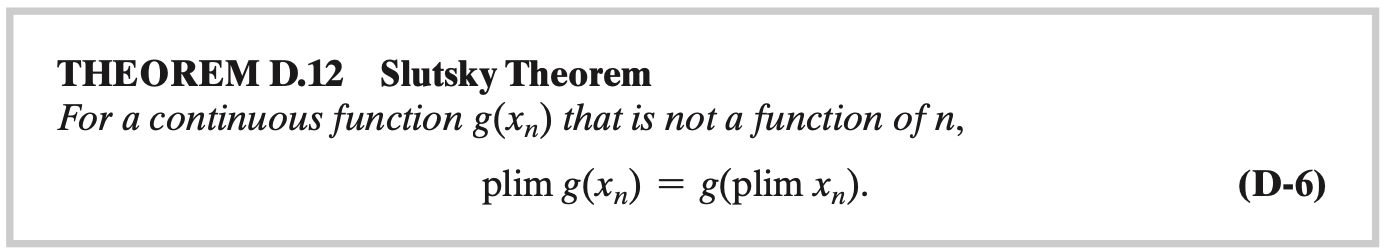
\includegraphics{/Users/henriquefonseca/Desktop/temp/Rmarkdown-practice/henriqueveras.github.io/files/Econometrics/Lecture Notes/3/theorem_d.6.png}
\end{frame}

\begin{frame}{Asymptotic Distribution of a Function of \(\mathbf{b}\):
The Delta Method}
\protect\hypertarget{asymptotic-distribution-of-a-function-of-mathbfb-the-delta-method-1}{}
According to the Slutsky Theorem,

\[\text{plim } f(\mathbf{b})= f(\text{plim } \mathbf{b})=f(\mathbf{\beta})\]

and

\[\text{plim } \mathbf{C}(\mathbf{b})=\frac{\partial f(\mathbf{\beta})}{\partial \mathbf{\beta}'}=\mathbf{\Gamma}\]
\end{frame}

\begin{frame}{Asymptotic Distribution of a Function of \(\mathbf{b}\):
The Delta Method}
\protect\hypertarget{asymptotic-distribution-of-a-function-of-mathbfb-the-delta-method-2}{}
Using a linear Taylor series approach, we expand this set of functions
in the approximation

\[f(\mathbf{b})= f(\mathbf{\beta})+\mathbf{\Gamma}\times (\mathbf{b}-\mathbf{\beta})+\text{higher order terms}\]

\vfill

The higher order terms become negligible in large samples if
\(\text{plim } \mathbf{b}=\mathbf{\beta}\).

\vfill

Thus the asymptotic distribution of the LHS of the above expression is
the same as the asymptotic distribution of the RHS.
\end{frame}

\begin{frame}{Asymptotic Distribution of a Function of \(\mathbf{b}\):
The Delta Method}
\protect\hypertarget{asymptotic-distribution-of-a-function-of-mathbfb-the-delta-method-3}{}
The mean of the asymptotic distribution is
\(\text{plim } f(\mathbf{b})=f(\mathbf{\beta})\) and the asymptotic
covariance matrix is
\[\mathbf{\Gamma}[Asy.Var(\mathbf{b}-\mathbf{\beta})]\mathbf{\Gamma}'\].

\vfill

These results are displayed in the theorem below.

\vfill

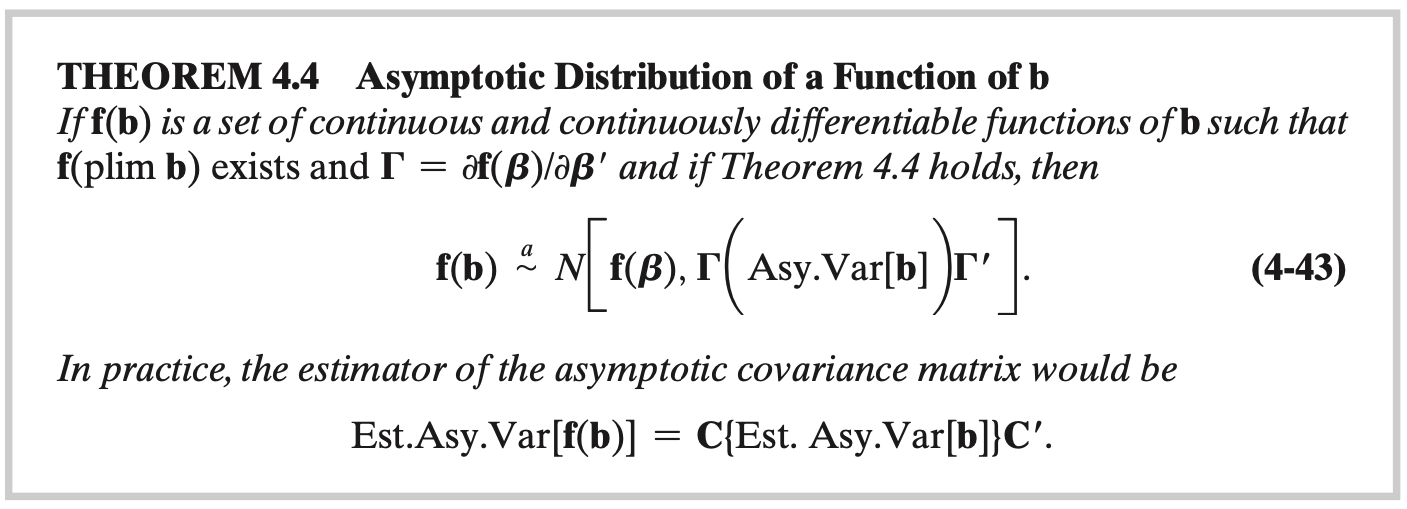
\includegraphics{/Users/henriquefonseca/Desktop/temp/Rmarkdown-practice/henriqueveras.github.io/files/Econometrics/Lecture Notes/3/theorem_4.4.png}
\end{frame}

\begin{frame}{An Example: The US gasoline market}
\protect\hypertarget{an-example-the-us-gasoline-market}{}
Suppose we are interested in estimating the short- and long-run impacts
of changes in price and income on the demand for gasoline.

\vfill

We can estimate the following model:

\[\begin{split}
ln(G/Pop)_t = & \beta_1+\beta_2 ln P_{G,t}+\beta_3 ln (Income/Pop)_t+\beta_4 lnP_{nc,t} \\ 
 & + \beta_5 lnP_{uc,t}+\gamma ln(G/Pop)_{t-1}+\varepsilon_t\end{split}\]

\vfill

In the short-run, price and income elasticities are \(\beta_2\) and
\(\beta_3\), respectively.

\vfill

In the long-run, equilibrium would require
\(ln(G/Pop)_t=ln(G/Pop)_{t-1}\).

\vfill

Therefore, long-run elasticities are \(\phi_2=\frac{\beta_2}{1-\gamma}\)
and \(\phi_3=\frac{\beta_3}{1-\gamma}\)

\vfill

How do we estimate these elasticities?
\end{frame}

\begin{frame}{An Example: The US gasoline market}
\protect\hypertarget{an-example-the-us-gasoline-market-1}{}
The LS estimates of the long-run elasticities are
\(f_2=b_2/(1-c)=-0.411\) and \(f_3=b_3/(1-c)=0.9705\).

\vfill

The estimated results are shown in the table below.

\vfill

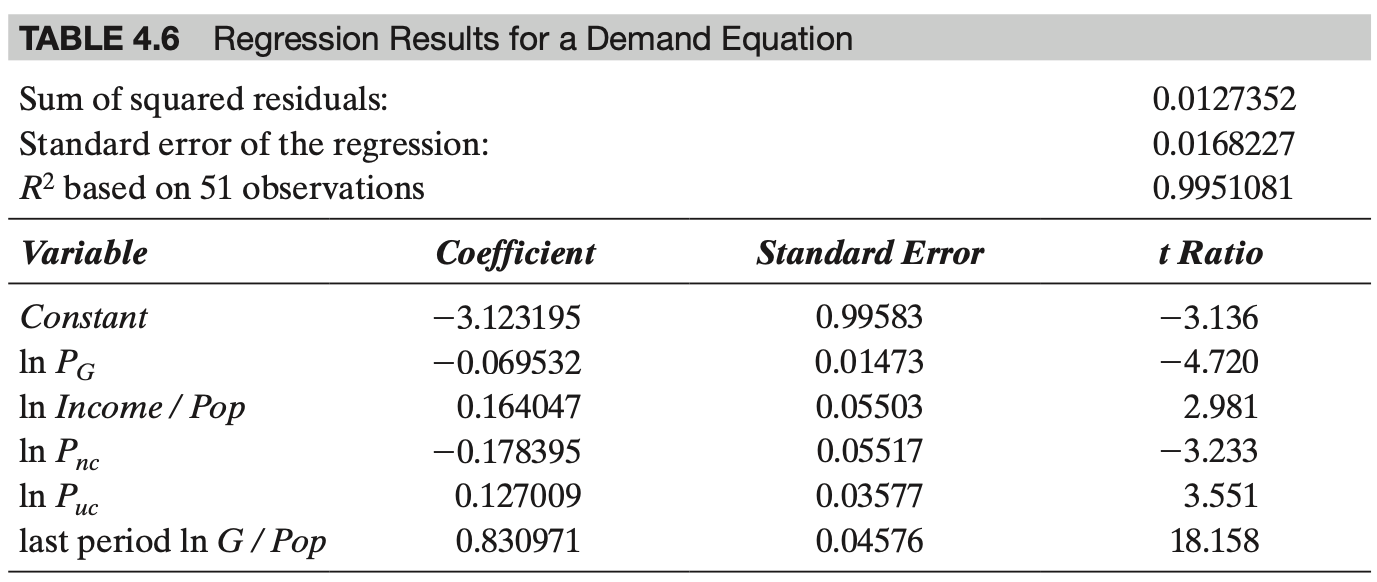
\includegraphics{/Users/henriquefonseca/Desktop/temp/Rmarkdown-practice/henriqueveras.github.io/files/Econometrics/Lecture Notes/3/table_4.6.png}
\end{frame}

\begin{frame}{An Example: The US gasoline market}
\protect\hypertarget{an-example-the-us-gasoline-market-2}{}
The next step is to estimate the standard errors of \(\phi_2\) and
\(\phi_3\).

\vfill

Recall the estimated asymptotic variance matrix obtained in theorem 4.4:
\[[\mathbf{C}[Asy.Var(\mathbf{b})]\mathbf{C}']=\mathbf{C}s^2(\mathbf{X'X})^{-1}\mathbf{C}'\]

\vfill

This yields

\vfill

\[Es.Asy.Va[b_2/(1-c)]=0.0231\]

\[Es.Asy.Va[b_3/(1-c)]=0.0264\]

\vfill

The (asymptotic) standard errors are the square roots 0.1522 and 0.1623,
respectively.

\vfill
\end{frame}

\hypertarget{interval-estimation}{%
\subsection{Interval Estimation}\label{interval-estimation}}

\begin{frame}{Interval Estimation}
\protect\hypertarget{interval-estimation-1}{}
The objective of interval estimation is to present the best estimate of
a parameter with an explicit expression of the uncertainty attached to
that estimate.

\vfill

A general approach would be
\[\hat{\theta}\pm \text{sampling variability}\]

\vfill

Consider two (uninformative) extreme cases:

\begin{enumerate}
\tightlist
\item
  100\% of confidence that the true population parameter lies in the
  range \(\hat{\theta}\pm \infty\)
\item
  0\% of confidence that the true population parameter lies in the range
  \(\hat{\theta}\pm 0\)
\end{enumerate}

\vfill

The objective is to choose a value \(\alpha\) such that we can attach
the confidence \(100(1-\alpha)\%\) to the interval.
\end{frame}

\begin{frame}{Forming a Confidence Interval for a Coefficient}
\protect\hypertarget{forming-a-confidence-interval-for-a-coefficient}{}
If \(\varepsilon|\mathbf{X} \sim N(0,\sigma^2\mathbf{I})\), then any
particular element of \(\mathbf{b}\) is distributed as

\[\mathbf{b}_k|\mathbf{X} \sim N(\mathbf{\beta}_k, \sigma^2 S^{kk})\]

where \(S^{kk}\) denotes the \(k\)th diagonal element of
\((\mathbf{X'X})^{-1}\).

\vfill

By standardizing the variable, we find

\[z_k=\frac{b_k-\beta_k}{\sqrt{\sigma^2S^{kk}}}\]

has a standard normal distribution.

\vfill

Using \(\alpha=0.05\), we know that
\(Prob[-1.96\leq z_k \leq 1.96]=0.95\).

\vfill
\end{frame}

\begin{frame}{Forming a Confidence Interval for a Coefficient}
\protect\hypertarget{forming-a-confidence-interval-for-a-coefficient-1}{}
By simple manipulation, we have

\[Prob[b_k-1.96\sqrt{\sigma^2 S^{kk}} \leq \beta_k \leq b_k+1.96\sqrt{\sigma^2 S^{kk}}]=0.95\]

\vfill

But recall that \(\sigma^2\) is unknown. Thus, we use \(s^2\) as its
estimator. Then, the ratio

\[t_k=\frac{b_k-\beta_k}{\sqrt{s^2S^{kk}}}\]

has a \(t\) distribution with \(n-K\) degrees of freedom (why?).
\end{frame}

\begin{frame}{Forming a Confidence Interval for a Coefficient}
\protect\hypertarget{forming-a-confidence-interval-for-a-coefficient-2}{}
If the disturbances do not follow a normal distribution, then the theory
for the \(t\) distribution does not apply.

\vfill

However, we can use the large sample results to find the \emph{limiting}
distribution of the statistic

\[z_k=\frac{\sqrt{n}(b_k-\beta_k)}{\sqrt{\sigma^2Q^{kk}}}\]

is standard normal, where \(\mathbf{Q}=\text{plim }(\mathbf{X'X}/n)\)
and \(Q^{kk}\) is the \(k\)th diagonal element of \(\mathbf{Q}^{-1}\).

\vfill

We can use \(s^2\) as a consistent estimator for \(\sigma^2\) and
estimate \(\mathbf{Q}^{-1}\) with \((\mathbf{X'X}/n)^{-1}\).
\end{frame}

\begin{frame}{Forming a Confidence Interval for a Coefficient}
\protect\hypertarget{forming-a-confidence-interval-for-a-coefficient-3}{}
This gives us precisely the \(t\) statistic for the exact distribution
case.

\vfill

To compute the confidence interval, however, we use the standard normal
distribution table rather than the \(t\) distribution.

\vfill

In practice, however, if the degrees of freedom are moderately large,
say greater than 100, the \(t\) distribution converges to the standard
normal one.

\vfill

The confidence interval would then be given by

\[Prob[b_k-1.96\sqrt{Est.Asy. Var(b_k)} \leq \beta_k \leq b_k+1.96\sqrt{Est.Asy. Var(b_k)}]=1-\alpha\]

\vfill
\end{frame}

\begin{frame}{Confidence Interval for a Linear Combination of
Coefficients: The Oaxaca's Decomposition}
\protect\hypertarget{confidence-interval-for-a-linear-combination-of-coefficients-the-oaxacas-decomposition}{}
Oaxaca (1973) and Blinder (1973) provide an application on how to form a
confidence interval for a linear function of the parameters.

\vfill

Let \(\mathbf{w}\) denote a \(K\times 1\) vector of known constants.

\vfill

Then, the linear combination \(c=\mathbf{w'b}\) is asymptotically
normally distributed with mean \(\gamma=\mathbf{w'\beta}\) and variance
\[\sigma^2_c=\mathbf{w}'[Asy. Var(\mathbf{b})]\mathbf{w}\] which we
estimate with \(s^2_c=\mathbf{w}'[Est.Asy. Var(\mathbf{b})]\mathbf{w}\).

\vfill

The confidence interval for \(\gamma\) is thus

\[Prob[c-z_{(1-\alpha /2)}s_c \leq \gamma \leq c-z_{(1-\alpha /2)}s_c]=1-\alpha\]
\end{frame}

\begin{frame}{The Oaxaca-Blinder Decomposition}
\protect\hypertarget{the-oaxaca-blinder-decomposition}{}
Consider Oaxaca's (1973) application, in the context of labor supply.

\vfill

The underlying regression model for men and women, separately, are

\[\ln wage_{m,i}=\mathbf{x}_{m,i}\beta_m+\varepsilon_{m,i}\]

\[\ln wage_{f,i}=\mathbf{x}_{f,i}\beta_f+\varepsilon_{f,i}\]

where \(\mathbf{x}_i\) includes sociodemographic variables, such as age,
education, and experience.

\vfill

The purpose is to compute both equations by decomposing the estimated
difference in wages in two components:

\begin{enumerate}
\tightlist
\item
  Differences in the levels of each observable variable of the model;
\item
  Differences in the (unexplained) ``effects''.
\end{enumerate}

\vfill
\end{frame}

\begin{frame}{The Oaxaca-Blinder Decomposition}
\protect\hypertarget{the-oaxaca-blinder-decomposition-1}{}
From the population regression equations, we have

\[\begin{split}
E[\ln wage_{m,i}|\mathbf{x}_{m,i}]-E[\ln wage_{f,i}|\mathbf{x}_{f,i}] & = \mathbf{x}_{m,i}\beta_m - \mathbf{x}_{f,i}\beta_f \\
 & = \mathbf{x}_{m,i}\beta_m - \mathbf{x}_{m,i}\beta_f + \mathbf{x}_{m,i}\beta_f - \mathbf{x}_{f,i}\beta_f \\
 & = \mathbf{x}_{m,i}(\beta_m - \beta_f) + (\mathbf{x}_{m,i}-\mathbf{x}_{f,i})\beta_f
\end{split}\]

\vfill

Assuming labor markets respond to differences in human capital properly,
the second term captures differences in human capital \emph{levels}
across both groups.

\vfill

The first term shows the differential in \(\log\) wages that is
attributed to differences unexplainable by human capital.

\vfill
\end{frame}

\begin{frame}{The Oaxaca-Blinder Decomposition}
\protect\hypertarget{the-oaxaca-blinder-decomposition-2}{}
We are interested in forming a confidence interval for the first term.
For this, we assume that both \(\mathbf{x}_m\) and \(\mathbf{x}_f\) are
known and we have two independent set of observations.

\vfill

Evaluating the model at the mean of the regression vectors,
\(\bar{\mathbf{x}}_m\) and \(\bar{\mathbf{x}}_f\), we find that
\(\mathbf{b}_m\) and \(\mathbf{b}_f\) are independent with means
\(\mathbf{\beta}_m\) and \(\mathbf{\beta}_f\) and estimated asymptotic
covariance matrices \(Est.Asy.Var[\mathbf{b}_m]\) and
\(Est.Asy.Var[\mathbf{b}_f]\).

\vfill

We are, then, forming a confidence interval for
\(\bar{\mathbf{x}}_m\mathbf{d}\), where
\(\mathbf{d}=\mathbf{b}_m-\mathbf{b}_f\). The estimated covariance
matrix is

\[Est.Asy.Var[\mathbf{d}]=Est.Asy.Var[\mathbf{b}_m]+Est.Asy.Var[\mathbf{b}_f]\].

\vfill

The CI will be constructed as before.

\vfill
\end{frame}

\hypertarget{prediction}{%
\subsection{Prediction}\label{prediction}}

\begin{frame}{Prediction \(\times\) Forecasting}
\protect\hypertarget{prediction-times-forecasting}{}
\textbf{Prediction}: Using the regression model to compute fitted
(predicted) values of the dependent variables (used in cross sections,
panel data, time series)

\vfill

\textbf{Forecasting} Same exercise, but explicitly giving role to time
and the purpose of the model building is to forecast future outcomes
(used in time series only).
\end{frame}

\begin{frame}{Prediction Intervals}
\protect\hypertarget{prediction-intervals}{}
Suppose we wish to predict the value of \(y^0\) associated with a
regressor vector \(\mathbf{x}^0\).

\vfill

The actual value would be

\[y^0=\mathbf{x}^{0'}\mathbf{\beta}+\varepsilon^0\]

\vfill

The prediction error is

\[e^0=\hat{y}^0-y^0=(\mathbf{b}-\mathbf{\beta})'\mathbf{x}^0-\varepsilon^0\]

\vfill
\end{frame}

\begin{frame}{Prediction Intervals}
\protect\hypertarget{prediction-intervals-1}{}
The prediction variance is

\[Var[e^0|\mathbf{X},\mathbf{x^0}]=Var[(\mathbf{b}-\mathbf{\beta})-\varepsilon^0|\mathbf{X},\mathbf{x^0}]=\sigma^2+\mathbf{x^0}'[\sigma^2(\mathbf{X'X})^{-1}]\mathbf{x^0}\]

\vfill

The prediction variance can be estimated by using \(s^2\) in place of
\(\sigma^2\).

\vfill

A confidence (prediction) interval for \(y^0\) would then be formed
using

\[y^0\pm t_{(1-\alpha /2), [n-K]}se(e^0)\]
\end{frame}


\section[]{}
\frame{\small \frametitle{Table of Contents}
\tableofcontents}
\end{document}
